\subsection{Analysis of Docking Scores}
Previous 4D docking work on agonist-bound AR informed selection of the receptor ensemble, which comprised PDB entries 2AMB, 2AM9, 3L3X, 2PNU, 2AXA, and 2AX9 following StructureProfiler quality assessment \cite{park2010improved,meyder2019structureprofiler,pereira2006comparison,zhou2010identification,cantin2007structural,bohl2005structural}. Co-crystallised ligands were redocked across the ensemble to assess the performance of the docking workflow and establish receptor-specific reference docking scores (Table~\ref{tab:ar_redocking_scores}). The control ligands produced scores ranging from $-27.85$ to $-13.25$, with a mean of $-20.23 \pm 5.16$. Compound 889 scored $-15.15$, which fell within the observed control range and one standard deviation of the control mean, whereas compound 681 scored $-32.77$, outside the control range.

\begin{table}[htbp]
    \centering
    \small
    \caption{Docking scores obtained by redocking the co-crystallised AR ligands across the selected receptor ensemble and by docking compounds 681 and 889. More negative docking scores indicate more favourable predicted binding within the scoring function.}
    \label{tab:ar_redocking_scores}
    \begin{tabular}{l c}
        \hline
        \textbf{Compound} & \textbf{Docking Score} \\
        \hline
        BHM (2AX9) & $-13.25$ \\
        DHT (3L3X) & $-16.72$ \\
        FHM (2AXA) & $-19.41$ \\
        TES (2AM9) & $-20.27$ \\
        ENM (2PNU) & $-23.89$ \\
        17H (2AMB) & $-27.85$ \\
        \hline
        Compound 681 & $-32.77$ \\
        Compound 889 & $-15.15$ \\
        \hline
    \end{tabular}
\end{table}

\subsection{Interactions and Visual Analysis}
Both compounds 681 and 889 formed $\pi$--$\pi$ interactions with Trp741 and showed their preferred docking poses in the 2PNU receptor conformation, in which Trp741 adopts a flipped orientation that accommodates the analogous interaction formed by the co-crystallised ligand ENM (Figure~\ref{fig:ar-interaction-analysis}A). In contrast to ENM, neither compound reproduced the key hydrogen-bonding interactions observed in the AR binding pocket. To assess pose similarity, compounds 681 and 889 were superimposed with ENM in the 2PNU binding site. Both compounds adopted broadly similar orientations to ENM (Figures~\ref{fig:ar-interaction-analysis}B and \ref{fig:ar-interaction-analysis}C), supporting the plausibility of the predicted binding poses despite the absence of these hydrogen-bonding contacts.


\begin{figure}[htbp]
    \centering

    \begin{subfigure}[b]{0.88\textwidth}
        \centering
        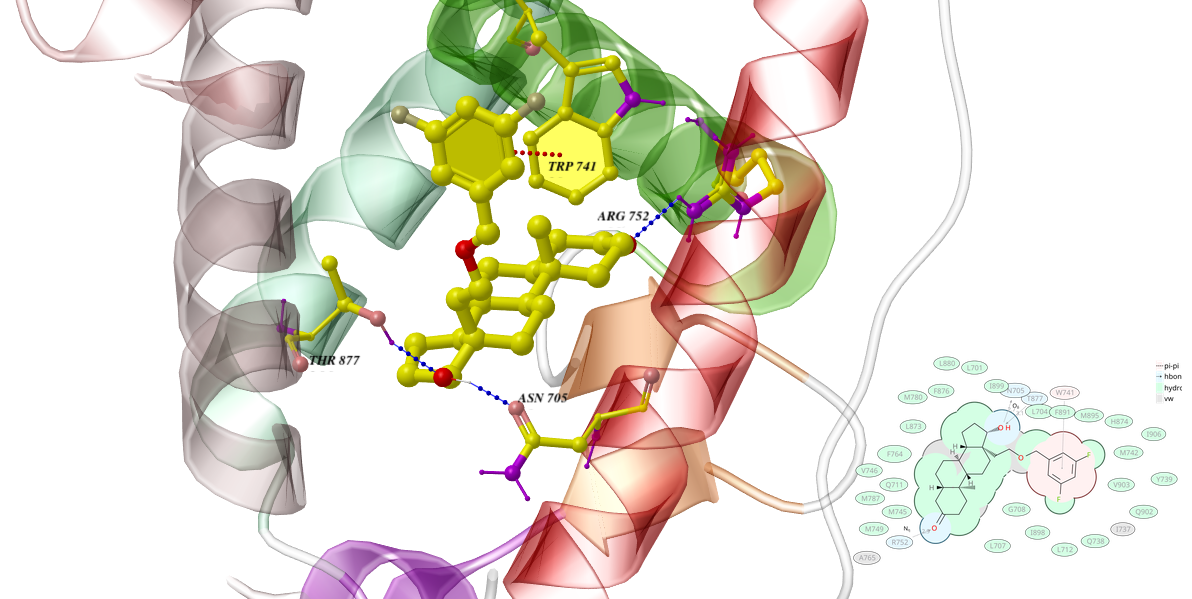
\includegraphics[width=\textwidth]{AR/combined/enm_2pnu.png}
        \caption{ENM (yellow) in the 2PNU AR conformation.}
        \label{fig:ar-enm}
    \end{subfigure}

    \vspace{0.8cm}

    \begin{subfigure}[b]{0.88\textwidth}
        \centering
        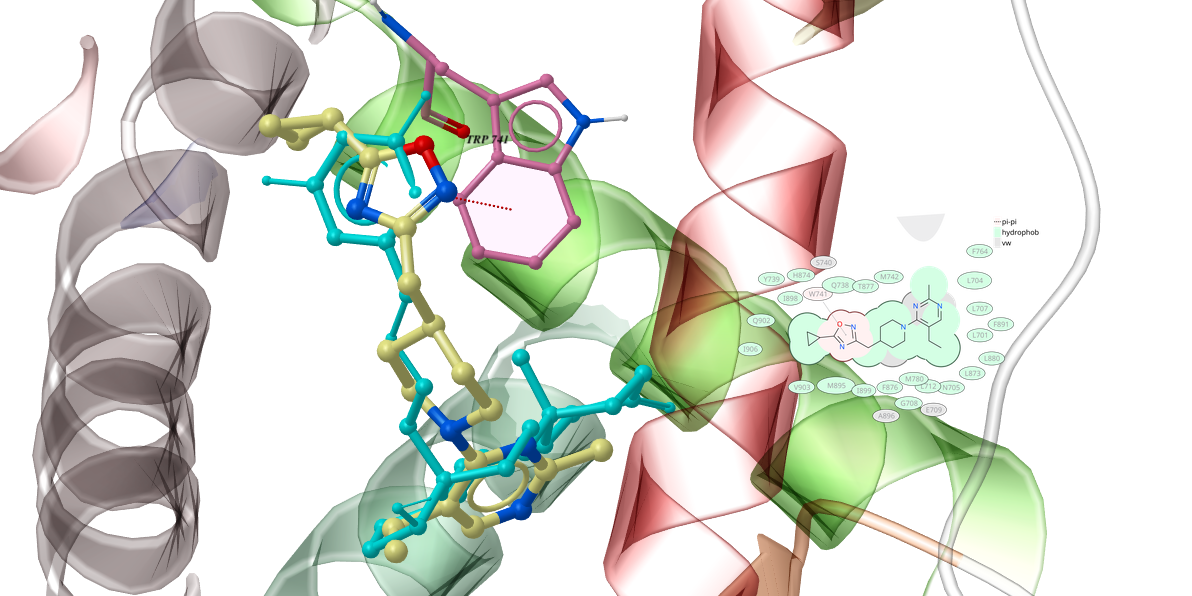
\includegraphics[width=\textwidth]{AR/combined/enm_sup_a.png}
        \caption{Compound 681 (yellow) superimposed with ENM (blue).}
        \label{fig:ar-681-superimposition}
    \end{subfigure}

    \vspace{0.8cm}

    \begin{subfigure}[b]{0.88\textwidth}
        \centering
        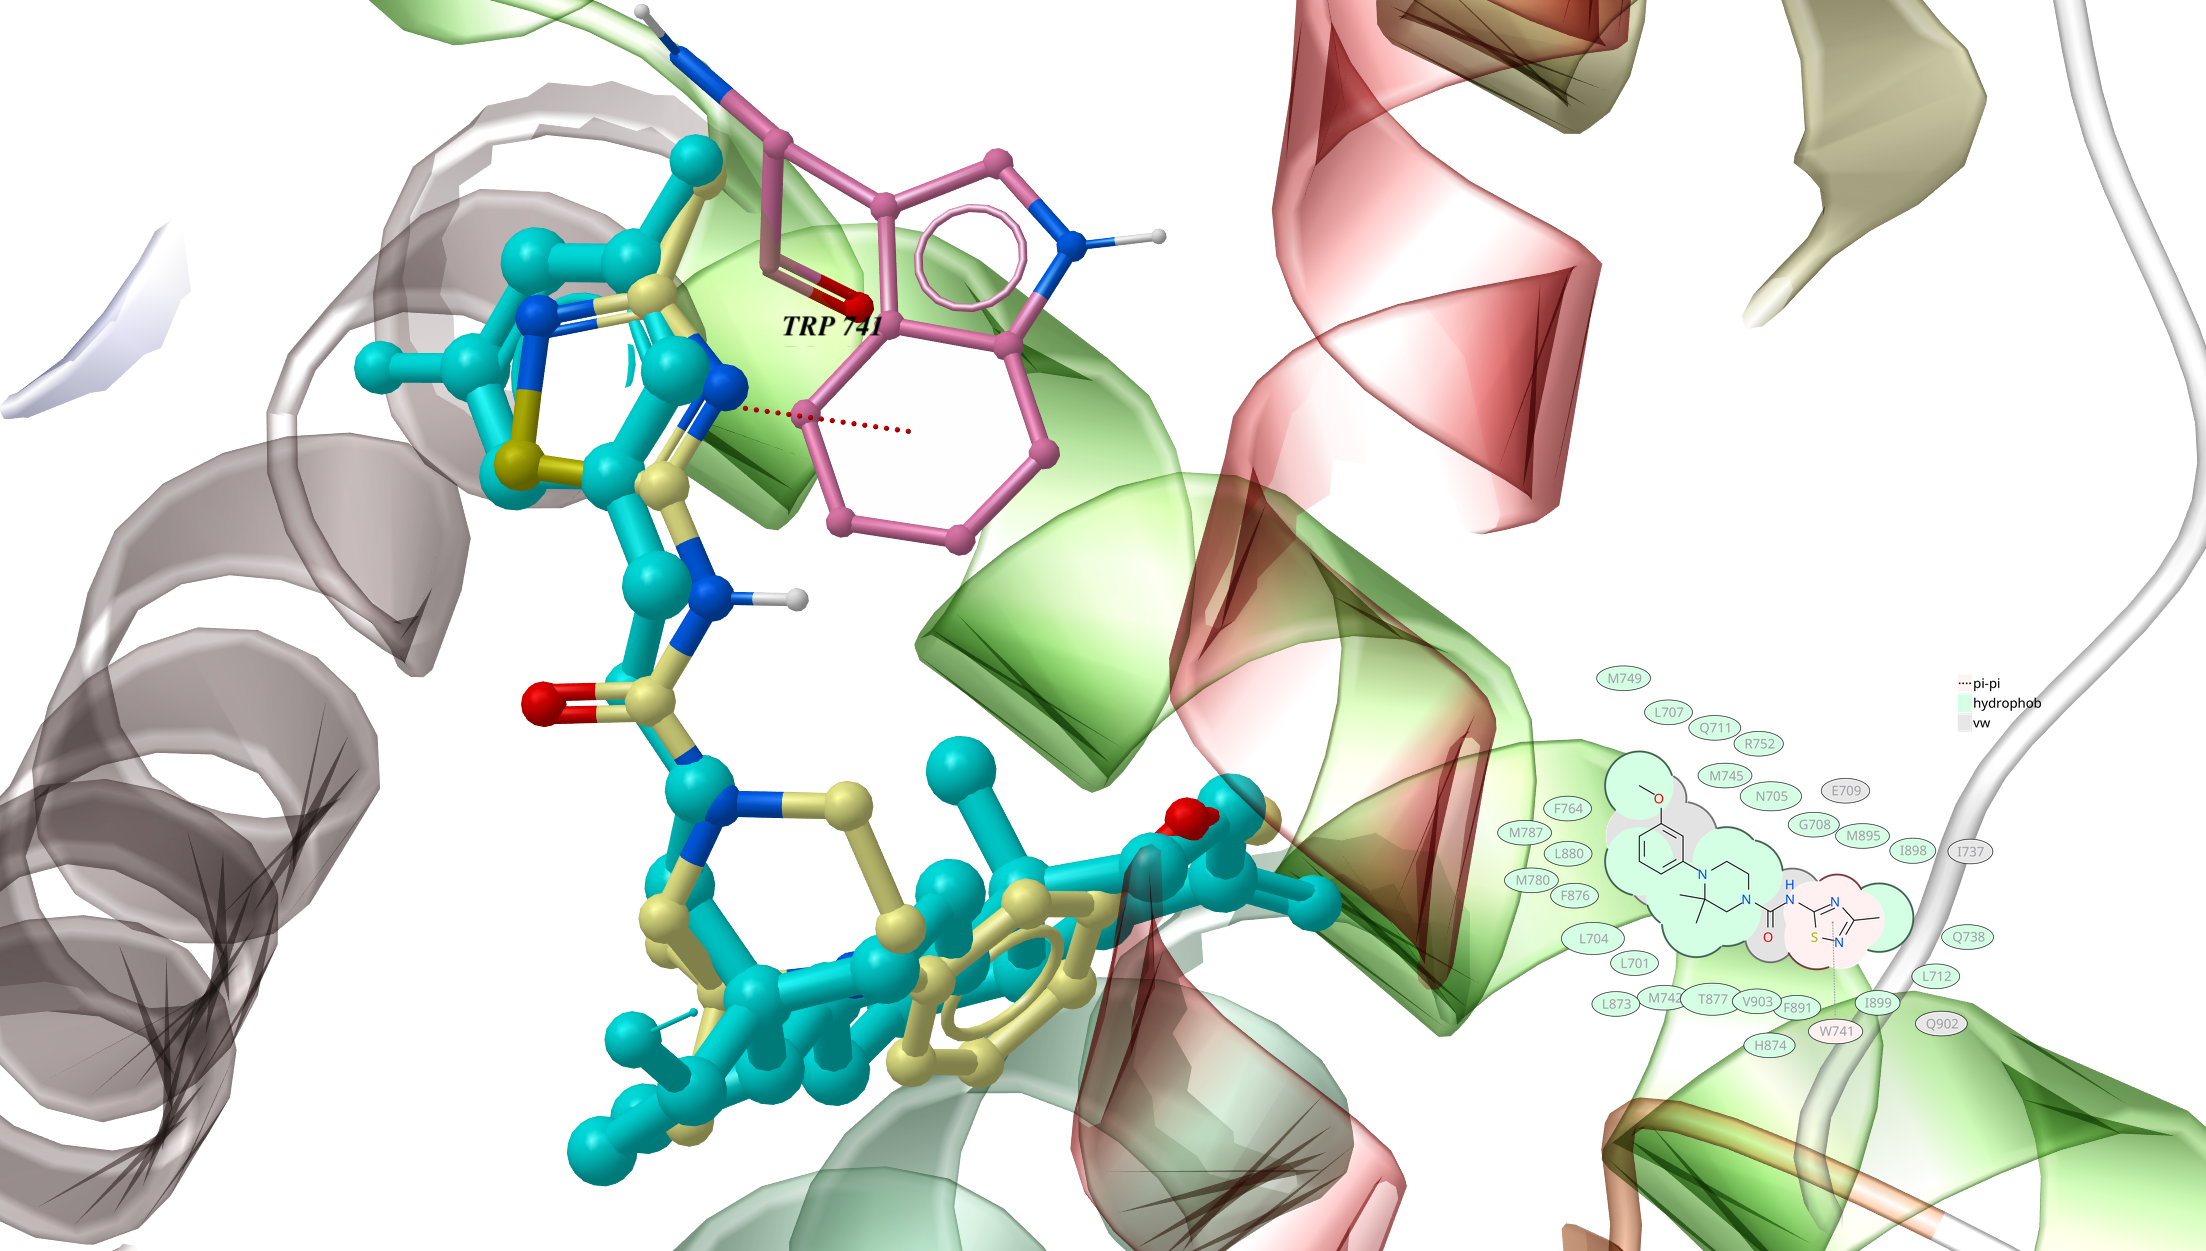
\includegraphics[width=\textwidth]{AR/combined/enm_sup_b.png}
        \caption{Compound 889 (yellow) superimposed with ENM (blue).}
        \label{fig:ar-889-superimposition}
    \end{subfigure}

    \caption{Visual comparison of predicted AR binding poses in the 2PNU receptor conformation. Hydrogen bonds are represented by blue dashed lines, whereas $\pi$--$\pi$ interactions are represented by red lines. The corresponding 2D interaction diagram is displayed at the bottom right of each 3D binding-pose view.}
    \label{fig:ar-interaction-analysis}
\end{figure}